In this section, we empirically evaluate STOIC's performance on executing machine learning application, comparing to single-runtime systems. We first outline the machine learning application benchmark that we consider and our experimental methodology. The result is then presented.

\subsection{Benchmark Application and Dataset}

We benchmark STOIC using an image processing application that classifies animal images from a wildlife monitoring system called Where's The Bear (WTB)~\cite{ref:wtb}. WTB is an end-to-end distributed data acquisition and analytics system that implements an IoT architecture and edge cloud. Our application inferences streaming photos taken by wildly deployed camera traps in Sedgwick Natural Reserve using a convolutional neural network (CNN)~\cite{ref:cnn} model trained by labeled images from the WTB dataset. Technically, it employs Tensorflow~\cite{ref:tensorflow} and Scikit-learn~\cite{ref:scikit} machine learning frameworks to perform the image classification.  

 In total, there are five classes that we consider in the CNN model training: Bird, Fox, Rodent, Human and Empty. Since the volume of classes are unbalanced due to different occurring frequency of animals, we up-sample the minority class (e.g. fox) by Keras ImageDataGenerator~\cite{ref:keras} to ensure the classifying model is not biased. Every image in the WTB dataset is resized to $1920 \times 1080$, and for each class, the dataset contains 251 images used to train CNN model. Once the model is trained, the application caches this model in hdf5 format and store it both at Edge Cloud disk storage and a shared volume in Ceph file system at Nautilus Cloud. 

\subsection{Application Efficacy}

\begin{figure}[t] \centering 
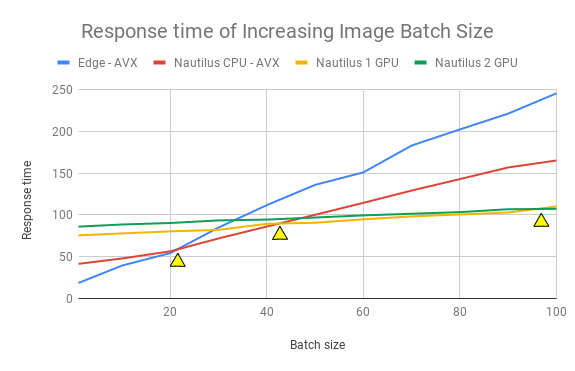
\includegraphics[scale=0.4]{response-time}
\caption{Response time of increasing batch size
\label{fig:response-time}}
\end{figure}

We first test the efficacy of STOIC by a series of image batches scheduled at four runtimes individually. The progressive response times are depicted in the Figure~\ref{fig:response-time}. The x-axis is the size of image batch and the y-axis The blue curve represents the linearly increasing response time from Edge Cloud runtime. The red one depicts the CPU runtime at Nautilus Cloud and its slope is more moderate since the CPU of node in Nautilus Cloud usually more powerful than Edge Cloud. The leftmost golden triangle marks cross point (21 images) of these two runtimes. When the batch size beyond the cross point, the scheduler should designate the task to \textit{cpu} runtime instead of \textit{edge}. Likewise, other two golden triangles mark cross points of \textit{cpu} / \textit{gpu1} (42 images) and \textit{gpu1} / \textit{gpu2} (95 images). According to the result, we ensure STOIC increases system performance by dynamic scheduling based on image batch size.

\subsection{Empirical Experiment}

To evaluate STOIC, we measure the total response time of multiple image batches processed by STOIC, comparing with four single runtimes. To accelerate the repetitive experiment, we developed a simulator to generate image batches based on the frequency distribution of WTB dataset. According to 2016 WTB dataset, the size of image batch fits to normal distribution $\mathbf{N}(\mu = 42.75, \sigma^2 = 39.5)$. Thus, the simulator generates images in the Edge Cloud to emulate batches from camera traps.

In the experiment setup, each experiment composes 24 batches, which is one day's worth of image from open field. To ensure the validity of outcome, We run such experiment 10 times for each runtime scenario and report the result. Table~\ref{tab:hybrid} lists the average value of total response time, total images and process time per image for individual runtime and STOIC. In the comparison, STOIC clearly has the lowest average process time per image in our experiment. This result indicates that STOIC outperforms four single-runtime scheduling mechanism in terms of response time.  

\begin{table}[t] \centering 
\scriptsize
\resizebox{\columnwidth}{!}{
\begin{tabular}{|c|c|c|c|} 
\hline
& \textbf{Avg. Resp time (sec)} & \textbf{Avg. Images} & \textbf{Process time/image (sec)} \\
\hline
edge & 3069.689 & 1217 & 2.52 \\
\hline
cpu & 1748.092 & 1095 & 1.59 \\
\hline
gpu1 & 1839.986 & 1113 & 1.65 \\
\hline
gpu2 & 2175.957 & 909 & 2.40 \\
\hline
STOIC & 1508.196 & 978 & \textbf{1.55} \\
\hline
\end{tabular}
}
\caption{Total Response time of 24 batches
\label{tab:hybrid}}
\end{table}



